\section{Neural networks}
On peut voir chaque couche du réseau de neurone comme un vecteur:
\textcolor{blue}{$$[a_0^{(0)}+a_1^{(0)} + a_2^{(0)} + a_3^{(0)} +...+ a_n^{(0)}]^T$$}
et chaque connection entre une couche et un neuron particulier vers la couche suivant comme une matrice de poids:

$$
\begin{bmatrix}
w_{0,0} & w_{0,1} &... &w_{0,n}\\
w_{1,0} & w_{1,1} &... &w_{1,n}\\
: & :   & ^{.}. & :\\
w_{n,0} & w_{n,1} &... &w_{n,n}\\
\end{bmatrix}$$}
 Ce que cela signifie, c'est de prendre la somme pondérée des activations dans la première couche en fonction de ces poids ?
$$
\sigma
\begin{pmatrix}
\textcolor{ao}{
\begin{bmatrix}
w_{0,0} & w_{0,1} &... &w_{0,n}\\
w_{1,0} & w_{1,1} &... &w_{1,n}\\
: & :   & ^{.}. & :\\
w_{n,0} & w_{n,1} &... &w_{n,n}\\
\end{bmatrix}}
\textcolor{blue}{
\begin{bmatrix}
a_0^{(0)}  \\
a_1^{(0)}  \\
:  \\
a_n^{(0)}  \\
\end{bmatrix}}
+
\textcolor{teal}{
\begin{bmatrix}
b_0  \\
b_1  \\
:  \\
b_n  \\
\end{bmatrix}}
\end{pmatrix}
= \begin{bmatrix}
a_0^{(1)}  \\
a_1^{(1)}  \\
:  \\
a_n^{(1)}  \\
\end{bmatrix}
$$
Dés lors, des qu'on à la connaisance du vecteur \textcolor{ao}{\textbf{w}} et du \biais \textcolor{teal}{\textbf{b}} on peut trouver la valeur du neuronnes suivants:
$$a_{(1)} = \sigma(\textcolor{ao}{\textbf{W}}a^{(0)} + \textcolor{teal}{\textbf{b})}$$

\subsection{La descente de gradient, ou comment un réseau de neuronal apprend}
Remember conceptually we're thinking of each neuron as beiing connected to all of the neurons in the previous layer and the weights in the weighted sum defining its activation are kind of like the strenghs of these connection and the bias is somme indication of wheter that neuron tends to be active or inactive and to start things off. We're just gonna initialize all of those weights and biaises totally randomely needless to say this network is going to perform pretty horribly on a given trainning example since it's just doing something random for example you feed in this image of a 3 and the output layer it just lokks like mess. So what you do is you define a cost function a way of telling the computer.\\
That output should have activations which are zero for most neurons, but one for this neuron what you gave me is utter trach. To say that more mathematically what you do is add up the squares of differances between each of these trash output activation and the value that you want them to have and this what we'll call the cost of single training example.\\
botice this sum is small when the network confidantly classifies the images correctly, but it's large when the network seems like it doesn't really what it's doing.

\subsection{Radials basis function network}
A neural network with a single hidden layer with Radial basis function as activations function.

  \begin{table}[!h]
    \begin{center}
    \begin{tabular}{| m{8em}|}
    \hline
    \rowcolor{vert.g} \textbf{Faster to train than MLP}    \\\hline
    \end{tabular}
    \end{center}
    \end{table}

\begin{figure}[H]
    \centering
    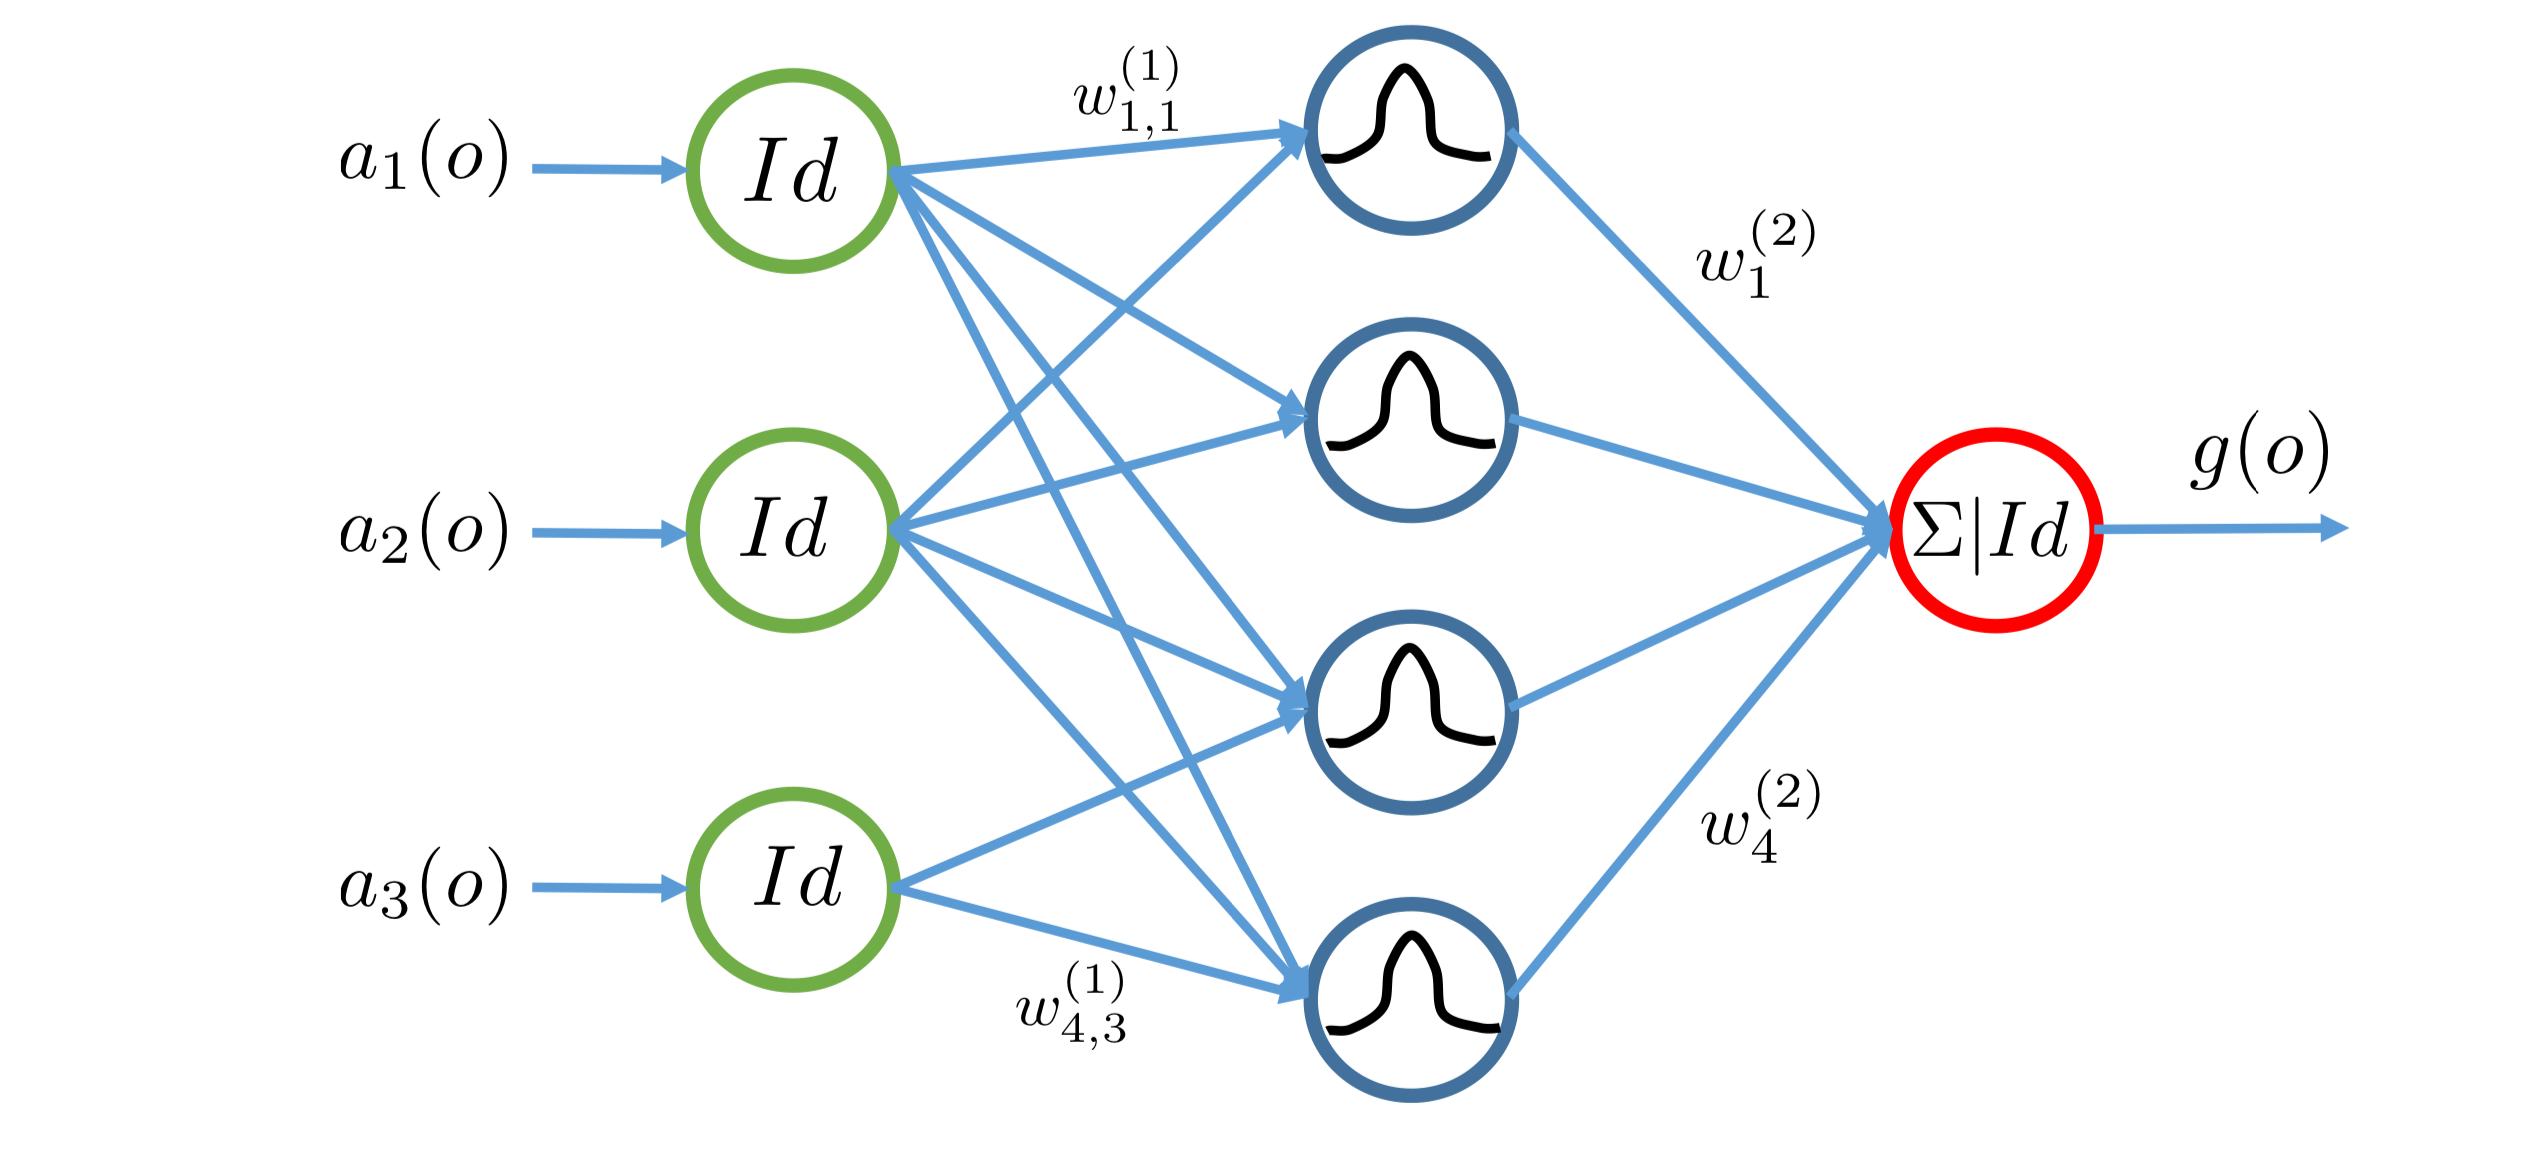
\includegraphics[scale = 0.3]{Question10/RadialBasisFunctionNetwork.png}
    \label{fig:my_label}
\end{figure}
  \subsection{Concolution NN} 
    \begin{table}[!h]
    \begin{center}
    \begin{tabular}{| m{8em}| m{15em}|}
    \hline
    \rowcolor{vert.g} \textbf{Concolutional Layer}     &  \begin{itemize}
                                                        \item Consiste of several layers where neurons are connected only to local re
                                                 \end{itemize}\\ \hline 
    \rowcolor{blue.g} \textbf{Pooling layer}       &  \begin{itemize}
                                                        \item \Each neuron is connected only to a local region (along width and height) at the same depth as its own depth in the previous layer
                                                 \end{itemize}\\ \hline
    \end{tabular}
    \end{center}
    \end{table}
    
        
    
    
        